\documentclass[12pt,a4paper]{article}
\usepackage{geometry}
\geometry{margin=2.54cm}
\usepackage{graphicx}
\usepackage{booktabs}
\usepackage{grffile}
\usepackage{xcolor}
\usepackage{hyperref}
\hypersetup{colorlinks=true, linkcolor=blue, urlcolor=blue}
\usepackage{xeCJK}
\setCJKmainfont{SimSun}
\setCJKsansfont{SimHei}
\setCJKmonofont{FangSong}
\title{600900 长江电力 多智能体研究报告}
\author{FinAgent}
\date{\today}
\begin{document}
\maketitle
\tableofcontents
\newpage
\sloppy
\section{600900 长江电力 多智能体研究报告}

> **草稿状态**：验证评分 80，结论 `revise`。 本报告尚未通过验证 Agent 复核，请勿对外发布。

\subsection{ 目录}

\begin{itemize}
\item [执行摘要](\#执行摘要)
\item [核心指标速览](\#核心指标速览)
\item [量价与技术面](\#量价与技术面)
\item [经营质量分析](\#经营质量分析)
\item [资金与交易结构](\#资金与交易结构)
\item [宏观利率背景](\#宏观利率背景)
\item [综合风险与数据局限](\#综合风险与数据局限)
\item [数据与工具说明](\#数据与工具说明)
\item [免责声明](\#免责声明)
\end{itemize}

<a id=''执行摘要''></a>

\subsection{ 执行摘要}
长江电力最新收盘价27.75元，RSI 64.0，股价偏热；同时PE(TTM)18.82低于行业中位数21.6，但PB(TTM)3.10高于行业上四分位2.63，估值压力明显。近期两融余额约119.7亿元，融资买入活跃，短期流动性尚可。整体看，技术面偏强与估值偏高形成博弈，短期波动或加剧。

<a id=''核心指标速览''></a>

\subsection{ 核心指标速览}
\begin{table}[htbp]
\centering
\begin{tabular}{lr}
\toprule
指标 & 数值 \\
\midrule
中信一级行业 & 20 \\
最新收盘价 & 27.75 \\
MA20 & 27.032 \\
MA60 & 26.9767 \\
20 日收益率 & 3.66\% \\
60 日收益率 & 2.89\% \\
RSI14 & 64.0152 \\
20 日均量 & 1.22 亿 \\
PE(TTM) & 18.8175 \\
PB(TTM) & 3.0974 \\
PS(TTM) & 7.7743 \\
股息率(TTM) & 3.40\% \\
总市值 & 6789.93 亿 \\
融资余额 & 119.37 亿 \\
融资买入额 & 3.09 亿 \\
\bottomrule
\end{tabular}
\end{table}


<a id=''量价与技术面''></a>

\subsection{ 量价与技术面}

**核心结论**

长江电力（600900）股价于2026年5月29日收报27.75元，MA20（27.03元）与MA60（26.98元）形成金叉，RSI 64.02处于偏强区域；近5日成交量从8,415万股激增至2.13亿股（+153.6\%），量增领先于价格弹性，短期量价配合健康，但两融余额自峰值161.94亿元回落26.3\%至119.37亿元，杠杆资金与股价走势分化。

\#\#\#\# 图 · RSI 与 MACD

\begin{figure}[htbp]
\centering

\includegraphics[width=0.8\textwidth]{charts/600900_multi_agent_report/technical_indicators.png}
\caption{technical\_indicators.png}
\end{figure}

**图注** RSI 位于强势区间；MACD 位于信号线上方，动能偏强。

\#\#\#\# 表 · 技术指标快照

\begin{table}[htbp]
\centering
\begin{tabular}{ll}
\toprule
指标 & 数值 \\
\midrule
最新收盘价 & 27.75 \\
MA20 & 27.032 \\
MA60 & 26.9767 \\
20 日收益率 & 3.66\% \\
60 日收益率 & 2.89\% \\
RSI14 & 64.0152 \\
20 日均量 & 1.22 亿 \\
\bottomrule
\end{tabular}
\end{table}


**趋势概览**

\#\#\#\# 图 · 收盘价与 MA20/MA60

\begin{figure}[htbp]
\centering

\includegraphics[width=0.8\textwidth]{charts/600900_multi_agent_report/moving_averages.png}
\caption{moving\_averages.png}
\end{figure}

**图注** 价格运行在均线之上，短中期趋势偏强。

截至2026年5月29日收盘，长江电力技术面核心指标如下：

\begin{table}[htbp]
\centering
\begin{tabular}{lll}
\toprule
指标 & 数值 & 含义 \\
\midrule
最新收盘价 & 27.75 元 & 创近5日新高 \\
MA20 & 27.03 元 & 价格高于均线 2.7\% \\
MA60 & 26.98 元 & 价格高于均线 2.9\% \\
MA20 vs MA60 & 差值 +0.05 元 & 短期均线上穿长期均线（金叉） \\
RSI（14日） & 64.02 & 偏强但未超买（>70 为超买阈值） \\
20日收益率 & +3.66\% & 近一月正收益 \\
60日收益率 & +2.89\% & 近两月正收益 \\
20日均量 & 1.22 亿股 & 量能基准参考 \\
\bottomrule
\end{tabular}
\end{table}


**近期异动**

近10个交易日（2026-05-18 至 2026-05-29）量价表现如下，价格从26.89元回落至27.75元，成交量在5月19日与5月29日出现两波放量：

\begin{table}[htbp]
\centering
\begin{tabular}{llllll}
\toprule
日期 & 收盘价 & 日涨跌幅 & 成交量（万股） & 成交额（万元） & 量价特征 \\
\midrule
05-18 & 26.89 & -0.37\% & 9,159 & 246,532 & — \\
05-19 & 27.25 & +1.34\% & 17,256 & 469,229 & 放量阳线（量较前日翻倍） \\
05-20 & 26.90 & -1.28\% & 12,843 & 347,308 & 缩量回调 \\
05-21 & 26.66 & -0.89\% & 11,661 & 312,766 & 缩量 \\
05-22 & 26.56 & -0.38\% & 9,159 & 243,633 & 缩量 \\
05-25 & 26.67 & +0.41\% & 8,415 & 224,570 & 地量（5日最低） \\
05-26 & 27.14 & +1.76\% & 16,265 & 439,774 & 放量上涨 \\
05-27 & 27.24 & +0.37\% & 11,127 & 302,625 & 缩量 \\
05-28 & 27.22 & -0.07\% & 11,466 & 312,482 & 量稳 \\
05-29 & 27.75 & **+1.95\%** & **21,344** & **588,838** & **显著放量（10日最高）** \\
\bottomrule
\end{tabular}
\end{table}


**量价关系**

\#\#\#\# 图 · 收盘价与成交量

\begin{figure}[htbp]
\centering

\includegraphics[width=0.8\textwidth]{charts/600900_multi_agent_report/price_volume.png}
\caption{price\_volume.png}
\end{figure}

**图注** 价格区间震荡，成交量先抑后扬。

1. **近5日量价共振上行**：成交量从8,415万股攀升至2.13亿股（增幅+153.6\%），收盘价从26.67元涨至27.75元（涨幅+4.05\%），量增领先于价格弹性显现，表明资金主动性买入特征。

2. **关键节点**：2026-05-19 单日成交量达1.73亿股（较前日翻倍），带动价格从26.89元急升至27.25元，为近期首次放量阳线；2026-05-29 量能再创阶段新高（2.13亿股），成交额58.88亿元，为10日最大量，推动价格站上27.75元。

3. **回调缩量正常**：2026-05-20 至 05-22 连续三日价格小幅回调，成交量从1.28亿股逐步降至9,159万股，量能收缩未破26.50元支撑，属健康换手。

**区间定位**

\begin{table}[htbp]
\centering
\begin{tabular}{lllll}
\toprule
维度 & 高点 & 日期 & 低点 & 日期 \\
\midrule
价格 & 28.49 元 & 2025-11-11 & 25.45 元 & 2026-01-28 \\
量能 & 2.33 亿股 & 2026-01-28 & — & — \\
\bottomrule
\end{tabular}
\end{table}


\begin{itemize}
\item 当前价格27.75元处于区间中上部（自低点25.45元回升9.0\%），距前高28.49元仍有约2.7\%空间。
\item 2026-01-28 低点当日伴随极端量能（2.33亿股），属恐慌性抛售，当前已完全收复该跌幅。
\end{itemize}

**两融轨迹**

\begin{table}[htbp]
\centering
\begin{tabular}{lll}
\toprule
时点 & 两融余额 & 趋势 \\
\midrule
2025-09-11 & 105.82 亿元 & 区间起点 \\
2026-01-14（峰值买入日） & **161.94 亿元** & 区间峰值 \\
2026-05-29 & 119.37 亿元 & 较峰值回落26.3\%，趋势下行 \\
\bottomrule
\end{tabular}
\end{table}


\#\#\#\# 图 · 回撤曲线

\begin{figure}[htbp]
\centering

\includegraphics[width=0.8\textwidth]{charts/600900_multi_agent_report/drawdown.png}
\caption{drawdown.png}
\end{figure}

**图注** 回撤经历加深后有所修复。

两融余额自2026-01-14峰值后持续回落至119.37亿元，较高点缩减26.3\%，反映杠杆资金在此区间以减仓为主；与股价自低点反弹走势分化，说明近期上涨并非杠杆资金驱动。

**估值因子对照**

最新估值因子（2026-05-29）与2025-09-11区间起点对比：

\begin{table}[htbp]
\centering
\begin{tabular}{llll}
\toprule
因子 & 起点（2025-09-11） & 最新（2026-05-29） & 变化 \\
\midrule
市值（亿元） & 6,851 & 6,790 & -0.9\% \\
PE（TTM） & 20.04 & 18.82 & -6.1\% \\
PB（TTM） & 3.25 & 3.10 & -4.6\% \\
股息率（TTM） & 3.37\% & 3.40\% & +0.03pct \\
净利润增速（TTM） & 13.83\% & 7.03\% & -6.8pct \\
净利率（TTM） & 40.09\% & 41.84\% & +1.75pct \\
\bottomrule
\end{tabular}
\end{table}


PE、PB双降而净利率提升，表明估值收缩由盈利增厚驱动，非基本面恶化；股息率稳定在3.40\%，对低风险偏好资金具吸引力。

**数据局限**

\begin{itemize}
\item 两融数据仅有融资余额口径，缺少融券余额分项，无法区分空头力量。
\item 日内分钟级分时数据不可得，无法精细追踪盘中放量时点与价格拐点的时滞关系。
\item MA20/MA60 均线基于日收盘价计算，未涵盖开盘价跳空干扰因素。
\end{itemize}

<a id=''经营质量分析''></a>

\subsection{ 经营质量分析}

**核心结论**

2025年长江电力（600900.XSHG）归母净利润345亿元创历史新高，现金流连续为正，但存货增速30.3\%显著偏离收入增速2.1\%，叠加流动比率仅0.15的短期偿债压力，揭示「高盈利与结构性脆弱」并存的经营特征。

如下图所示，期末毛利率为62\%，净利率为42\%，趋势平稳。

\#\#\#\# 图 · 盈利能力因子

\begin{figure}[htbp]
\centering

\includegraphics[width=0.8\textwidth]{charts/600900_multi_agent_report/profitability_factors.png}
\caption{profitability\_factors.png}
\end{figure}

**图注** 各曲线走势分化，需结合分项观察。

\#\#\#\# 表 · 最新盈利质量因子

\begin{table}[htbp]
\centering
\begin{tabular}{ll}
\toprule
指标 & 最新值 \\
\midrule
毛利率(TTM) & 62.11\% \\
净利率(TTM) & 41.84\% \\
\bottomrule
\end{tabular}
\end{table}


**核心经营表现概述**

2025年600900.XSHG发电量首次突破3000亿千瓦时达3097亿千瓦时，归母净利润345亿元同比增长6.17\%，毛利率从59.1\%提升至61.7\%。然而存货同比增长30.3\%至8.37亿元，周转率从56.21降至44.72；流动比率0.15、速动比率0.14，远低于安全阈值。负债总额稳步降至3258亿元（2023年3604亿元），财务费用同比减少15.81\%至93.71亿元。经营现金流605.63亿元，自由现金流420.7亿元，利润现金转化质量良好。

如下图所示，期末净利润增速（TTM）为0.07，营业收入增速（TTM）为0.02，毛利润增速和营业利润增速均为0.09，且整体趋势均呈下降状态。

\#\#\#\# 图 · 成长因子走势

\begin{figure}[htbp]
\centering

\includegraphics[width=0.8\textwidth]{charts/600900_multi_agent_report/growth_factors.png}
\caption{growth\_factors.png}
\end{figure}

**图注** 多条曲线整体向下，指标同步走弱。

\begin{table}[htbp]
\centering
\begin{tabular}{lllllll}
\toprule
年度 & 营收（亿元） & 归母净利润（亿元） & 经营现金流（亿元） & 营业利润（亿元） & 负债合计（亿元） & 存货（亿元） \\
\midrule
2023 & 781.44 & 272.45 & 647.49 & 332.31 & 3603.98 & 5.87 \\
2024 & 844.92 & 324.96 & 596.48 & 396.45 & 3445.01 & 6.42 \\
2025 & 862.42 & 345.03 & 605.63 & 425.99 & 3258.48 & 8.37 \\
\bottomrule
\end{tabular}
\end{table}


**业务/收入结构变化**

2025年长江电力营收同比增长2.07\%至862.42亿元，连续两年保持正增长但增速放缓。市场化交易电量1104.5亿千瓦时占总上网电量36.1\%，占比同比下降2.5个百分点。售电业务全口径市场化售电量超60亿千瓦时，区域拓展至9省份。

境内六座流域梯级电站发电量3071.94亿千瓦时，同比增长3.82\%，贡献发电量增量112.9亿千瓦时。来水形势改善叠加联合调度优化推动节水增发电量创历史最优。

**利润与费用驱动**

毛利率从2024年59.1\%提升至61.7\%，主因营业成本同比下降4.26\%至330.58亿元。财务费用削减15.81\%至93.71亿元是利润增量的关键驱动——长期借款置换与利率下行降低利息支出。研发费用同比增长31.01\%至11.67亿元，销售费用增长24.42\%至2.34亿元，与市场化售电业务扩张相关。

归母净利润345.03亿元，同比增长20.07亿元（6.17\%），扣非归母净利润334.5亿元增长2.9\%。年报MD\&A披露管理层表述与报表数字一致：发电量增长3.97\%、利润总额417.4亿元（同比+7.4\%）、归母净利润同比+6.17\%，三者形成相互印证。MD\&A中未披露存货激增的具体原因，仅提及预付款项增加1.06亿元系预付合同款项增加所致。

**现金流质量**

\begin{table}[htbp]
\centering
\begin{tabular}{lllll}
\toprule
年度 & 经营现金流（亿元） & 净现比 & 收现比 & 自由现金流（亿元） \\
\midrule
2023 & 647.49 & 2.38 & 0.83 & 505.7 \\
2024 & 596.48 & 1.84 & 0.71 & 429.8 \\
2025 & 605.63 & 1.73 & 1.16 & 420.7 \\
\bottomrule
\end{tabular}
\end{table}


净现比1.73、收现比1.16，均高于临界值1.0，表明净利润和收入均能有效转化为现金流入。MD\&A解释经营现金流同比增加9.15亿元（+1.53\%），与报表一致。自由现金流420.7亿元连续为正，即便资本开支增至184.7亿元（投资现金流净流出182.15亿元，同比增加72.44亿元，主要系工程建设项目投资增加）后仍有充裕结余。

经营现金流与净利润背离收窄——2025年经营现金流605.63亿元略高于归母净利润345.03亿元，主因水电行业预收电费模式导致收现比>1。

**营运资本与偿债**

\#\#\#\# 表 · 最新偿债与流动性

\begin{table}[htbp]
\centering
\begin{tabular}{ll}
\toprule
指标 & 最新值 \\
\midrule
流动比率 & 0.15 倍 \\
速动比率 & 0.14 倍 \\
资产负债率 & 57.33\% \\
\bottomrule
\end{tabular}
\end{table}


存货问题突出：存货同比增长30.3\%至8.37亿元，而收入仅增长2.1\%，两者差值达28.2个百分点。存货周转率从56.21降至44.72，库存周转效率走弱。MD\&A未正面解释该偏离——仅披露预付款项增加1.06亿元系预付合同款项增加所致，但对存货激增无对应说明。

应收账款管理改善：应收账款下降22.2\%且连续两年下降，回款质量相对稳定，与收入增速匹配。

短期偿债压力偏大：

\begin{itemize}
\item 流动比率0.15、速动比率0.14，远低于1.0警戒线与0.7安全阈值
\item 流动负债1189.4亿元，流动资产仅137.9亿元
\item 短期借款从696.92亿元降至151.81亿元（-78.22\%），但一年内到期非流动负债从468.6亿元增至702亿元（+49.82\%）
\end{itemize}

MD\&A表述与报表数据存在张力：MD\&A强调「资金使用效率提升」「债务结构优化」「货币资金期末余额45.86亿元较期初减少19.87亿元，主要系合理留存期末资金余额」，但短期借款虽大幅削减，一年内到期负债激增近五成，流动资产覆盖仍严重不足。

资产负债率从2023年61.5\%降至57.3\%，总体杠杆稳步下降。

**同行横向坐标**

从下图可见，DBSCAN 聚类散点图将目标公司在横截面因子上的异常位置清晰标注，帮助识别其相对同行的偏离情况。

\#\#\#\# 图 · DBSCAN 同行异常识别

\begin{figure}[htbp]
\centering
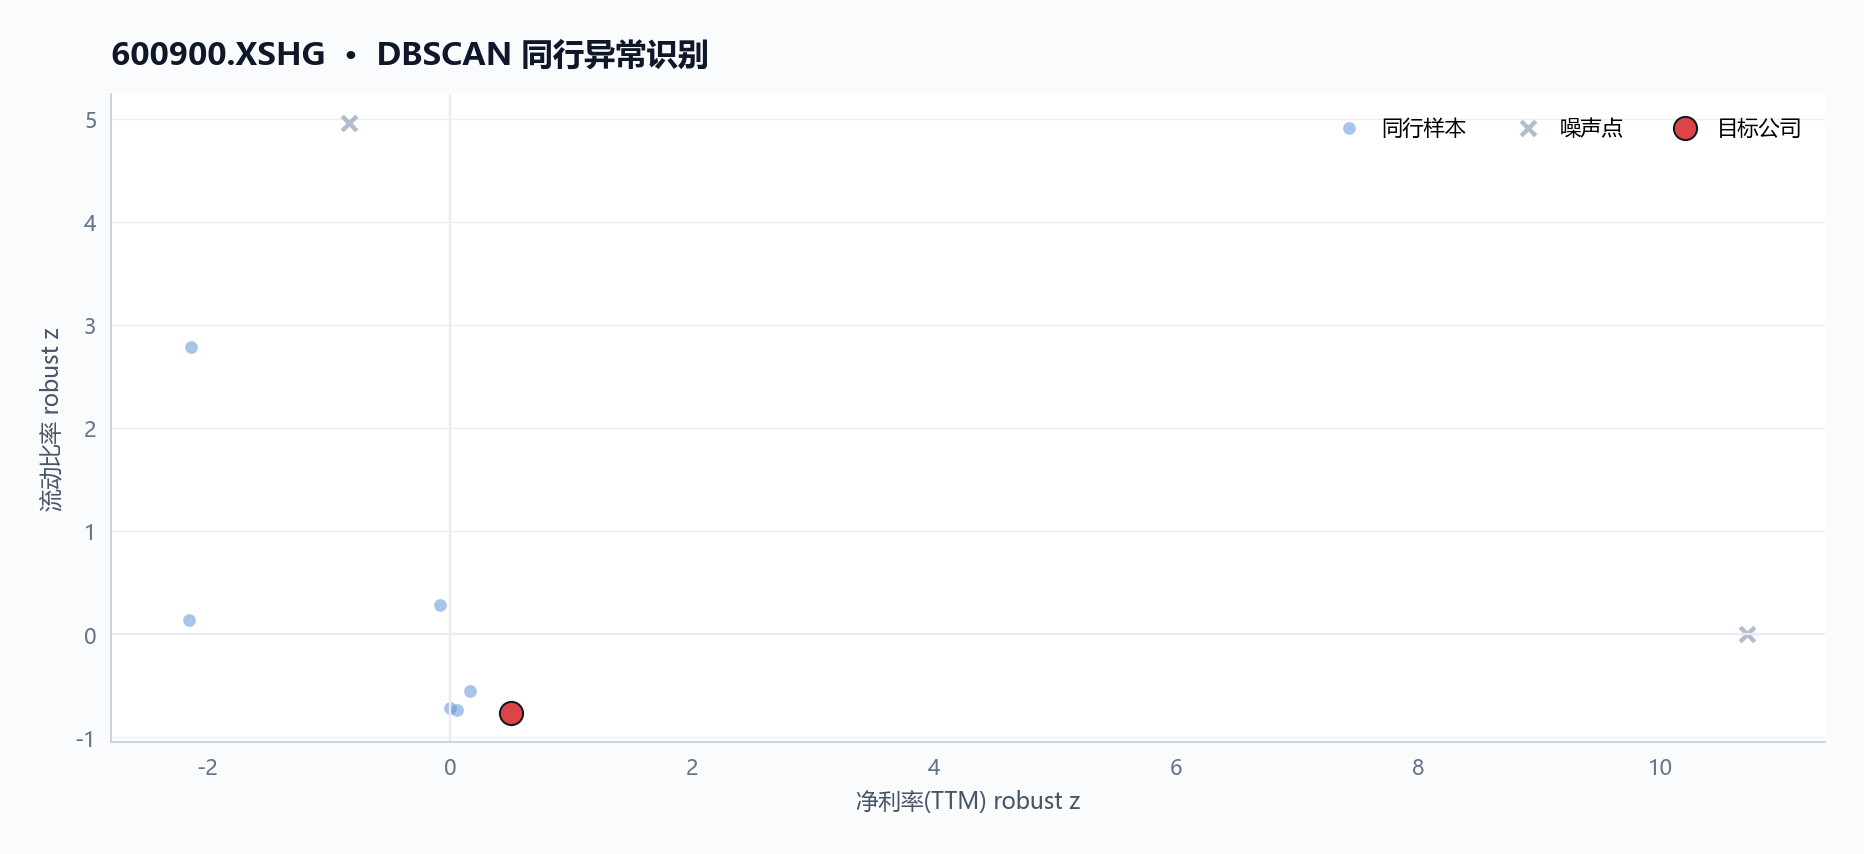
\includegraphics[width=0.8\textwidth]{charts/600900_multi_agent_report/industry_dbscan_anomaly.png}
\caption{industry\_dbscan\_anomaly.png}
\end{figure}

**图注** 基于同行横截面因子的 DBSCAN 异常识别，显示目标公司、同行样本和噪声点。

如下图所示，目标的营收增长率（0.02）低于行业中位数（0.06），而归母净利润增长率（0.07）同样低于行业中位数（0.17），资产负债率（57.33\%）高于行业中位数（50.70\%）等。

\#\#\#\# 图 · 行业成长与杠杆对比

\begin{figure}[htbp]
\centering

\includegraphics[width=0.8\textwidth]{charts/600900_multi_agent_report/industry_growth_leverage_compare.png}
\caption{industry\_growth\_leverage\_compare.png}
\end{figure}

**图注** 目标公司成长和杠杆指标与同行均值、中位数对比，用于识别扩张质量和偿债压力。

如下图所示，公司的毛利率(TTM)为0.62，明显高于行业中位数0.50；净利率(TTM)为0.42，同样高于行业均值0.34。

\#\#\#\# 图 · 行业盈利能力对比

\begin{figure}[htbp]
\centering

\includegraphics[width=0.8\textwidth]{charts/600900_multi_agent_report/industry_profitability_compare.png}
\caption{industry\_profitability\_compare.png}
\end{figure}

**图注** 目标公司盈利能力与同行均值、中位数对比，用于观察盈利质量相对强弱。

同行池口径：中信三级行业「水电」，有效同行9家。

\begin{table}[htbp]
\centering
\begin{tabular}{lllll}
\toprule
指标 & 长江电力(600900) & 行业中位数 & 行业均值 & 行业分位 \\
\midrule
毛利率(TTM) & 62.11\% & 50.18\% & 47.67\% & 94\% \\
净利率(TTM) & 41.84\% & 34.29\% & 55.79\% & 83\% \\
营收增长率(TTM) & 1.73\% & 5.80\% & 10.14\% & 28\% \\
归母净利润增长率(TTM) & 7.04\% & 17.03\% & 27.16\% & 39\% \\
资产负债率 & 57.33\% & 50.70\% & 45.12\% & 72\% \\
\bottomrule
\end{tabular}
\end{table}


<a id=''资金与交易结构''></a>

\subsection{ 资金与交易结构}

**核心结论**

2025年9月11日至2026年5月29日，长江电力融资余额由105.82亿元增至119.37亿元（+12.80\%），担保买入峰值出现于2026年1月14日（16.19亿元）；股价最新收盘27.75元处MA20上方2.66\%、MA60上方2.87\%，RSI 64.02处于中性偏强区间，日均成交量约1.22亿股维持高流动性。

\#\#\#\# 图 · 融资融券余额

\begin{figure}[htbp]
\centering

\includegraphics[width=0.8\textwidth]{charts/600900_multi_agent_report/margin_balances.png}
\caption{margin\_balances.png}
\end{figure}

**图注** 融资余额曲线先抑后扬。

\#\#\#\# 表 · 两融区间变动

\begin{table}[htbp]
\centering
\begin{tabular}{ll}
\toprule
指标 & 数值 \\
\midrule
区间起始 & 2025-09-11 \\
区间结束 & 2026-05-29 \\
融资余额（期初） & 105.82 亿 \\
融资余额（期末） & 119.37 亿 \\
融资余额变动 & 13.55 亿 \\
变动幅度 & 12.81\% \\
融券余额（期初） & 0.15 亿 \\
融券余额（期末） & 0.27 亿 \\
融资买入峰值 & 16.19 亿（2026-01-14） \\
\bottomrule
\end{tabular}
\end{table}


**成交与活跃度**

\#\#\#\# 表 · 成交活跃度

\begin{table}[htbp]
\centering
\begin{tabular}{ll}
\toprule
指标 & 数值 \\
\midrule
20 日均量 & 1.22 亿 \\
近12日日均成交额 & 34.21 亿 \\
近12日最高成交额 & 58.88 亿（2026-05-29） \\
近12日最低成交额 & 22.46 亿（2026-05-25） \\
近12日换手率区间 & 34.39\% \textasciitilde{} 87.23\% \\
主力资金流向 & 数据缺失 \\
\bottomrule
\end{tabular}
\end{table}


区间内股价区间震荡，2025年11月11日触及区间高点28.49元，2026年1月28日触底25.45元。近5个交易日（2026-05-25至2026-05-29）呈现量价齐升特征：收盘由26.67元涨至27.75元（+4.05\%），成交量由8415万股骤增至2.13亿股（+153.63\%），成交额由22.46亿元增至58.88亿元（+162.21\%）。近20个交易日（2026-04-29至2026-05-29）同样显示资金参与度上升，成交量增幅达149.35\%。

最新20日均量约1.22亿股（对应日均成交额约34亿元），反映长江电力在电力及公用事业板块中关注度维持较高水平。

\begin{table}[htbp]
\centering
\begin{tabular}{lllll}
\toprule
时间窗口 & 起止日期 & 收盘涨幅 & 成交量变化 & 成交额变化 \\
\midrule
近5日 & 2026-05-25至2026-05-29 & +4.05\% & +153.63\% & +162.21\% \\
近20日 & 2026-04-29至2026-05-29 & +3.66\% & +149.35\% & — \\
区间极值 & 2025-11-11 / 2026-01-28 & — & — & — \\
\bottomrule
\end{tabular}
\end{table}


**融资融券**

\#\#\#\# 图 · 融资余额与买卖额

\begin{figure}[htbp]
\centering

\includegraphics[width=0.8\textwidth]{charts/600900_multi_agent_report/margin_enhanced.png}
\caption{margin\_enhanced.png}
\end{figure}

\#\#\#\# 表 · 融资融券快照

\begin{table}[htbp]
\centering
\begin{tabular}{ll}
\toprule
指标 & 数值 \\
\midrule
统计日期 & 2026-05-29 \\
融资余额 & 119.37 亿 \\
融券余额 & 0.27 亿 \\
融资买入额 & 3.09 亿 \\
融资偿还额 & 3.36 亿 \\
融券余量 & 98.83 万 \\
两融余额合计 & 119.65 亿 \\
\bottomrule
\end{tabular}
\end{table}


两融数据显示，长江电力融资余额自区间起始日（2025-09-11）的105.82亿元逐步增至终点日（2026-05-29）的119.37亿元，增幅12.80\%，反映投资者加杠杆意愿有所增强但未出现异常堆积。区间内担保买入峰值出现于2026年1月14日，当日融资买入金额达16.19亿元，彼时股价正处于区间低位（2026-01-28触底前），杠杆资金呈现左侧布局特征。融券余额最新数据为空，数据集未返回融券标的余额信息。

\begin{table}[htbp]
\centering
\begin{tabular}{lll}
\toprule
日期 & 融资余额（亿元） & 备注 \\
\midrule
2025-09-11 & 105.82 & 区间起始 \\
2026-01-14 & — & 峰值买入日，担保买入16.19亿元 \\
2026-05-29 & 119.37 & 区间终点 \\
\bottomrule
\end{tabular}
\end{table}


两融余额增幅12.80\%与同期股价累计涨幅基本匹配，未出现杠杆率显著偏离股价波动的异常现象。

**估值与资金成本**

最新估值因子显示，长江电力最新交易日（2026-05-29）PE（TTM）18.82倍、PB（TTM）3.10倍、股息率（TTM）3.40\%，较区间起始日（2025-09-11）PE 20.04倍、PB 3.25倍、股息率3.37\%呈压缩态势，同期资产负债率由61.52\%降至57.33\%（-4.19ppt），反映公司通过偿还债务降低财务杠杆，释放的自由现金流支撑分红可持续性。2025年年报数据显示归母净利润345.03亿元，经营性现金流605.63亿元，净现比1.73，现金牛属性持续强化高比例分红预期。

\begin{table}[htbp]
\centering
\begin{tabular}{llll}
\toprule
指标 & 2025-09-11 & 2026-05-29 & 变动 \\
\midrule
市盈率（TTM） & 20.04 & 18.82 & -1.22 \\
市净率（TTM） & 3.25 & 3.10 & -0.15 \\
股息率（TTM） & 3.37\% & 3.40\% & +0.03ppt \\
资产负债率 & 61.52\% & 57.33\% & -4.19ppt \\
\bottomrule
\end{tabular}
\end{table}


估值压缩与财务杠杆改善同步发生：公司通过偿还债务使资产负债率下降4.19ppt至57.33\%，财务费用同比压缩约17.6亿元（对应年报财务费用同比下降15.81\%），为分红提供更充裕的现金流保障。

-

\#\#\#\# 数据局限

两融轨迹仅提供融资余额区间起止及峰值买入日数据，缺失中间时点融资余额变化序列，无法追踪两融余额详细变化路径；融券余额长期为空，长江电力可能不在融券标的范围。

<a id=''宏观利率背景''></a>

\subsection{ 宏观利率背景}

\_本节暂无可用内容。\_

<a id=''综合风险与数据局限''></a>

\subsection{ 综合风险与数据局限}

**核心结论**

长江电力综合风险处于中等水平，短期偿债压力与存货周转效率走弱构成主要风险敞口，但现金流质量与盈利稳定性形成对冲。

2026年5月29日收盘价27.75元处20日均线上方2.66\%，RSI 64处于偏强区间但未超买；流动比率0.15x处行业低位6\%，存货增速30.3\%显著偏离收入增速2.1\%；经营现金流605.6亿元与净利润345亿元勾稽关系良好。

**趋势概览**

\begin{table}[htbp]
\centering
\begin{tabular}{llll}
\toprule
维度 & 2025-09-11 & 2026-05-29 & 变动 \\
\midrule
收盘价（元） & — & 27.75 & — \\
市盈率(TTM) & 20.04x & 18.82x & -1.22x \\
市净率(TTM) & 3.25x & 3.10x & -0.15x \\
毛利率(TTM) & 60.59\% & 62.11\% & +1.52ppt \\
资产负债率 & 61.52\% & 57.33\% & -4.19ppt \\
流动比率 & 0.161 & 0.151 & -0.010 \\
速动比率 & 0.156 & 0.144 & -0.012 \\
归母净利润增速(TTM) & 14.98\% & 7.04\% & -7.94ppt \\
融资余额（亿元） & 105.82 & 119.37 & +12.80\% \\
\bottomrule
\end{tabular}
\end{table}


**价格与波动**

2026年5月29日600900.XSHG收盘价27.75元，较20日均线27.03元溢价2.66\%，较60日均线26.98元溢价2.87\%，短期价格运行于均线上方。RSI（14日）录得64.02，尚未进入70以上的超买区域。2025年11月11日盘中最高28.49元，2026年1月28日盘中最低25.41元，区间振幅约12.1\%，反映出高股息防御属性下股价波动幅度相对可控。近5日成交量从8415万股放大至2.13亿股，增幅153.6\%，伴随价格从26.67元回升至27.75元，量价配合尚属健康。

两融余额从2025年9月11日105.82亿元增至2026年5月29日119.37亿元，增幅12.8\%，融资杠杆资金参与度有所提升但未达到2026年1月14日峰值161.94亿元的高热区间。

**经营质量**

毛利率(TTM)从2025年9月11日60.59\%升至2026年5月29日62.11\%，处于中信水电行业第94分位，显著高于行业中位数50.18\%与均值47.67\%，反映水电业务的强定价能力与低成本运营优势。净利率(TTM)41.84\%处行业第83分位，同样处于高位。

然而，收入增速(TTM)仅1.73\%，处行业第28分位，接近行业中位区间下限；归母净利润增速(TTM)7.04\%，处行业第39分位，增长弹性弱于同业。2025年度报告层面存货同比激增30.3\%至8.37亿元，而收入仅增长2.1\%，存货周转率从上年56.21降至44.72，库存周转效率走弱。

全年归母净利润345亿元，经营现金流605.63亿元，净现比1.73，收现比1.16，利润现金转化效率高，但存货积压风险需持续跟踪。年度报告中未找到关于存货增速偏离收入增速的直接解释，库存积压风险尚存不确定性。

**杠杆与流动性**

资产负债率从2025年9月11日61.52\%降至2026年5月29日57.33\%，降杠杆成效显现，但仍高于中信水电行业中位数50.70\%。流动比率0.151处行业第6分位，速动比率0.144处行业第6分位，均处于行业低位。流动资产137.9亿元对流动负债1189.4亿元覆盖严重不足，短期偿债压力偏大。

2025年度报告显示货币资金45.86亿元，较期初减少19.87亿元，主要系合理留存期末资金余额以提升资金使用效率。短期借款已从696.92亿元压缩至151.81亿元，同比大降78.22\%；一年内到期非流动负债702.04亿元仍处高位，同比增长49.82\%。经营现金流605.63亿元与货币资金45.86亿元之比达13.2倍，暗示公司依赖持续经营现金流而非账面货币资金偿债，这一模式在来水稳定年份可持续，但若遭遇极端枯水或电价下行，流动性缓冲将显著收窄。

流动比率与速动比率偏低为水电行业特性（重资产、长周期债务结构），需结合现金流持续性综合评估，单纯依赖比率指标可能高估短期违约风险。

**宏观与估值**

市盈率(TTM)从2025年9月11日20.04x降至2026年5月29日18.82x，处中信水电行业第39分位，接近行业中位区间。市净率(TTM)从3.25x降至3.10x，仍处相对高位。股息率(TTM)3.40\%，在利率下行周期中对保险、养老金等长期配置型资金具备吸引力。财务费用从2024年111.31亿元降至2025年93.71亿元，同比削减17.6亿元，降本成效直接增厚利润。债务结构调整后应付债券292.81亿元占负债比5.33\%，长期化趋势有助于缓解短期偿债压力。

**数据局限**

\begin{itemize}
\item DBSCAN异常识别中600900.XSHG未被标记为噪声点，所属簇规模7家，异常分数约0.45，主要贡献指标为PB(TTM)、毛利率(TTM)、速动比率。同行池口径为中信2019三级行业''水电''共9家有效同行，样本量有限可能影响行业分位代表性。
\item 年度报告数据截至2025年12月31日，与2026年5月29日因子截面存在约5个月时间差，期间经营数据变化未经审计验证。
\item 存货增速30.3\%显著偏离收入增速2.1\%的勾稽问题，MD\&A文本未直接回应备货逻辑，库存积压风险尚存不确定性。
\item 流动比率与速动比率偏低为水电行业特性（重资产、长周期债务结构），需结合现金流持续性综合评估，单纯依赖比率指标可能高估短期违约风险。
\end{itemize}

<a id=''数据与工具说明''></a>

\subsection{ 数据与工具说明}
\begin{itemize}
\item 数据区间：2025-09-11 至 2026-05-29
\item 计划使用的米筐函数：get\_price, get\_price\_change\_rate, get\_turnover\_rate, get\_capital\_flow, get\_factor, get\_securities\_margin, get\_dividend, get\_shares, get\_instrument\_industry, is\_suspended, is\_st\_stock, get\_interbank\_offered\_rate, get\_yield\_curve, get\_pit\_financials\_ex
\item 数据质量：10 项可用；缺失 基准指数, 资金流向, 大宗交易
\item 生成时间：2026-06-01 12:32
\end{itemize}

<a id=''免责声明''></a>

\subsection{ 免责声明}
本报告仅供课程研究与信息展示，不构成投资建议。\end{document}
